\section{Zajímavé problémy}
\label{sec:zajimave-problemy}

Jednou z hlavních a oblíbených podmnožin diskrétní matematiky a kombinatoriky
je \emph{teorie grafů}. Jednoduše řečeno, graf je množina bodů -- vrcholů, mezi
některýmiž vedou spojnice -- hrany.

Představíme si pár úloh jako ze života, jak bývá v matematice zvykem, jejichž
zdánlivá nevinnost je v rozporu s jejich významem pro rozvoj teorie.

\subsection{Problém tří domů a tří studní}
\label{ssec:problem-tri-domu-a-tri-studni}

V zemi za sedmero horami a sedmero řekami žili byli tři sousedi. Každý z~nich
vlastnil rodinný domek a dělili se o vodu ze tří blízkých studní. Jednou se
ale sousedi po sporu rozkmotřili a už se nechtěli ani vidět. Potřebovali ale
pitnou vodu. Každý se odmítl vzdát nároku na nějakou ze studní, tak si jako
poslední společný čin najali dvorního architekta, by nechal postavit cesty od
každého domu ke každé studni. Cesty se nesměly nikde potkat, aby do sebe
sousedi na cestě pro vodu náhodou nenarazili.

Dvorní architekt, probděv tři dny a tři noci hledaje způsob, jak nasupené
sousedy uspokojit, klekl nakonec únavou a prohlásil, že cesty bez křížení
vystavět nelze.

My s ním souhlasíme, ale není lehké najít způsob, jak úlohu matematicky
formalizovat, a podat důkaz.

\begin{figure}[h]
 \centering
  \begin{tikzpicture}
  \path[use as bounding box] (-4, 2.5) rectangle (4, -2.5);
  \node[scale=2] (house2) at (0, 1) {\faHome};
  \node[scale=2, left=1cm of house2] (house1) {\faHome};
  \node[scale=2, right=1cm of house2] (house3) {\faHome};

  \node[scale=2, below=1cm of house2] (well2-outer) {\faCircleThin};
  \node[scale=1.2] (well2-inner) at (well2-outer.center) {\faCircle};

  \node[scale=2, left=1cm of well2-outer] (well1-outer) {\faCircleThin};
  \node[scale=1.2] (well1-inner) at (well1-outer.center) {\faCircle};

  \node[scale=2, right=1cm of well2-outer] (well3-outer) {\faCircleThin};
  \node[scale=1.2] (well3-inner) at (well3-outer.center) {\faCircle};

  \node[below=2mm of house1.center] (house1-door) {};
  \node[below=2mm of house2.center] (house2-door) {};
  \node[below=2mm of house3.center] (house3-door) {};

  \draw[thick] (house2-door.center) -- (well1-inner.north);
  \draw[thick] (house2-door.center) -- (well2-inner.north);
  \draw[thick] (house2-door.center) -- (well3-inner.north);

  \draw[thick] (house1-door.center) -- (well1-inner.north);
  \draw[thick] (house3-door.center) -- (well3-inner.north);
  
  \node[below left=.5mm of well2-inner.center] (well2-southwest) {};
  \node[below right=.5mm of well2-inner.center] (well2-southeast) {};

  \node[above right=.5mm of well1-inner.center] (well1-northeast) {};
  \node[above left=.5mm of well3-inner.center] (well3-northwest) {};

  \draw[thick] (house1-door.center) .. controls (-5, -3) and (-1, -2) ..
  (well2-southwest);
  \draw[thick] (house3-door.center) .. controls (5, -3) and (1, -2) ..
  (well2-southeast);

  \draw[thick] (house1-door.center) .. controls (-1, -2) and (-1, 6) ..
  (well3-inner.north);
  \draw[thick,dashed,red] (house3-door.center) -- (well1-northeast);
 \end{tikzpicture}
 \caption{Tři domy a tři studně.}
\end{figure}

\subsection{Hrátky s puntíky}
\label{ssec:hratky-s-puntiky}

Ukážeme si ještě dvě pěkné úlohy s puntíky a čarami. Mějme třeba deset puntíků
v rovině a pár z nich spojme čarami, jako na
\hyperref[fig:random-graph-on-10-pts]{obrázku~\ref*{fig:random-graph-on-10-pts}}.

\begin{figure}[h]
 \centering
 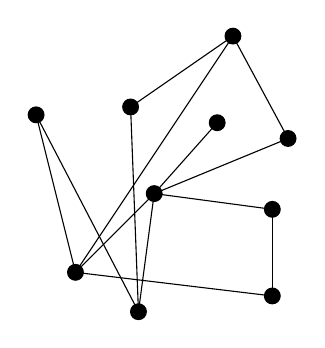
\begin{tikzpicture}
  \node[circle,draw,fill=black,minimum size=2mm,inner sep=0pt,outer sep=0pt]
  (v1) at (0, 0) {};
  \node[circle,draw,fill=black,minimum size=2mm,inner sep=0pt,outer sep=0pt]
  (v2) at (1, 2) {};
  \node[circle,draw,fill=black,minimum size=2mm,inner sep=0pt,outer sep=0pt]
  (v3) at (-1, -1) {};
  \node[circle,draw,fill=black,minimum size=2mm,inner sep=0pt,outer sep=0pt]
  (v4) at (-1.5, 1) {};
  \node[circle,draw,fill=black,minimum size=2mm,inner sep=0pt,outer sep=0pt]
  (v5) at (1.5, -1.3) {};
  \node[circle,draw,fill=black,minimum size=2mm,inner sep=0pt,outer sep=0pt]
  (v6) at (1.7, 0.7) {};
  \node[circle,draw,fill=black,minimum size=2mm,inner sep=0pt,outer sep=0pt]
  (v7) at (-0.2, -1.5) {};
  \node[circle,draw,fill=black,minimum size=2mm,inner sep=0pt,outer sep=0pt]
  (v8) at (0.8, 0.9) {};
  \node[circle,draw,fill=black,minimum size=2mm,inner sep=0pt,outer sep=0pt]
  (v9) at (-0.3, 1.1) {};
  \node[circle,draw,fill=black,minimum size=2mm,inner sep=0pt,outer sep=0pt]
  (v10) at (1.5, -0.2) {};

  \draw (v1) -- (v3);
  \draw (v1) -- (v6);
  \draw (v1) -- (v7);
  \draw (v1) -- (v8);
  \draw (v1) -- (v10);
  \draw (v2) -- (v3);
  \draw (v2) -- (v6);
  \draw (v2) -- (v9);
  \draw (v3) -- (v4);
  \draw (v3) -- (v5);
  \draw (v4) -- (v7);
  \draw (v5) -- (v10);
  \draw (v7) -- (v9);
 \end{tikzpicture}
 \caption{Náhodný graf na deseti vrcholech.}
 \label{fig:random-graph-on-10-pts}
\end{figure}

Otázka, kterou se budeme časem zabývat zní \uv{Kolik maximálně mohu nakreslit
spojnic, než mi vznikne trojúhelník?} Trojúhelníkem zde myslíme trojici bodů,
z nichž každé dva jsou spojeny. Do tohoto grafu se určitě ještě dají nějaké
přikreslit, ale kolik přesně? A jak tuto úlohu řešit obecně pro jakýkoliv
počet bodů?

Podobně zajímavá, ale už víc algoritmická otázka, by zněla \uv{Jak poznám,
jestli v nějakém grafu existuje trojúhelník?}. Samozřejmě by šlo se prostě
podívat na každou jednu trojici bodů, ale jde to i líp?

Ještě na pár odstavců zůstaneme u spojených puntíků. Úloha, která se ukázala
jako zásadní v teorii grafů má co dělat s cestami. \emph{Cestou} v grafu
nazveme posloupnost bodů -- vrcholů, takovou, že mezi sousedními vrcholy na
cestě vždycky vede spojnice. Jinak řečeno, mohu se v klidu projít od jednoho
vrcholu k druhému, aniž bych musel skákat mezi vrcholy. Naším úkolem je najít
takovou množinu spojnic -- hran, že se mezi každými dvěma vrcholy dá projít po
cestě.

Pro deset vrcholů jedno možné řešení vidíte na
\hyperref[fig:minimal-skeleton-on-10-pts]{obrázku
\ref*{fig:minimal-skeleton-on-10-pts}}.

\begin{figure}[h]
 \centering
 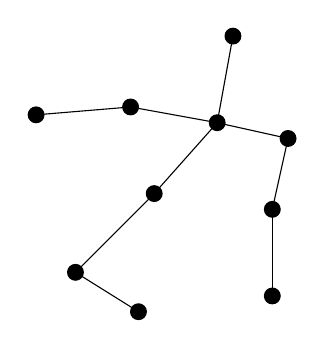
\begin{tikzpicture}
  \node[circle,draw,fill=black,minimum size=2mm,inner sep=0pt,outer sep=0pt]
  (v1) at (0, 0) {};
  \node[circle,draw,fill=black,minimum size=2mm,inner sep=0pt,outer sep=0pt]
  (v2) at (1, 2) {};
  \node[circle,draw,fill=black,minimum size=2mm,inner sep=0pt,outer sep=0pt]
  (v3) at (-1, -1) {};
  \node[circle,draw,fill=black,minimum size=2mm,inner sep=0pt,outer sep=0pt]
  (v4) at (-1.5, 1) {};
  \node[circle,draw,fill=black,minimum size=2mm,inner sep=0pt,outer sep=0pt]
  (v5) at (1.5, -1.3) {};
  \node[circle,draw,fill=black,minimum size=2mm,inner sep=0pt,outer sep=0pt]
  (v6) at (1.7, 0.7) {};
  \node[circle,draw,fill=black,minimum size=2mm,inner sep=0pt,outer sep=0pt]
  (v7) at (-0.2, -1.5) {};
  \node[circle,draw,fill=black,minimum size=2mm,inner sep=0pt,outer sep=0pt]
  (v8) at (0.8, 0.9) {};
  \node[circle,draw,fill=black,minimum size=2mm,inner sep=0pt,outer sep=0pt]
  (v9) at (-0.3, 1.1) {};
  \node[circle,draw,fill=black,minimum size=2mm,inner sep=0pt,outer sep=0pt]
  (v10) at (1.5, -0.2) {};
  
  \draw (v4) -- (v9);
  \draw (v9) -- (v8);
  \draw (v8) -- (v2);
  \draw (v8) -- (v6);
  \draw (v8) -- (v1);
  \draw (v1) -- (v3);
  \draw (v3) -- (v7);
  \draw (v6) -- (v10);
  \draw (v10) -- (v5);
 \end{tikzpicture}
 \caption{Minimální kostra grafu na deseti vrcholech.}
 \label{fig:minimal-skeleton-on-10-pts}
\end{figure}

Je jednoduché si rozmyslet, kolik nejméně hran je třeba nakreslit. Ovšem, co
když můžeme vybírat jen z nějaké předem dané množiny? Řešení pak nemusí vždycky
existovat (může se totiž stát, že žádné hrany k dispozici nemáme). Dá se nějak
efektivně poznat, kdy úlohu lze řešit a kdy ne? A co třeba otázka, kolik
existuje řešení s minimálním počtem hran; co řešení, součet přes všechny jehož
hrany je nejmenší? V této obecné podobě se úloze (i jejímu řešení) říká
\emph{minimální kostra} grafu a v budoucnu ji, stejně jako předchozí dvě úlohy,
potkáme.

